\chapter{Resultados} \label{cap:results}
Neste capítulo são apresentados os resultados obtidos do trabalho desenvolvido. Primeiramente, os resultados de negócio envolvidos na implementação da aplicação são apresentados. Em seguida, uma comparação das ferramentas de teste automatizado é feita. Por último, são discutidos os resultados obtidos do ponto de vista da empresa em que este projeto esteve inserido.

\section{Versão Piloto}
\subsection{Uso do Aplicativo}
O desenvolvimento do aplicativo para o sistema iOS, apresentado neste trabalho, culminou no lançamento da sua versão piloto. Esta versão consiste na primeira etapa de lançamentos do produto e tem como objetivo a validação da ideia. O aplicativo piloto foi avaliado por um grupo seleto de academias e treinadores, localizados em Sydney.

A Figura \ref{fig:pilot-use} ilustra a utilização da versão piloto do aplicativo, com dados coletados da ferramenta Fabric. O gráfico mostra o número de usuários ativos diariamente desde o lançamento do piloto. O eixo horizontal representa a evolução temporal em dias, enquanto o eixo vertical contém o número total de usuários diários. O primeiro pico (entre os dias 10 e 28 de outubro) corresponde a distribuição de um incremento da versão piloto, ultrapassando o número de 10 usuários. O segundo e o terceiro picos (entre os dias 4 e 11 de novembro) dizem respeito a uma nova versão de incremento do piloto, com o convite de mais parceiros para o teste do aplicativo. Totalizando 19 usuários utilizando a aplicação.

\begin{figure}[H]
    \centering
    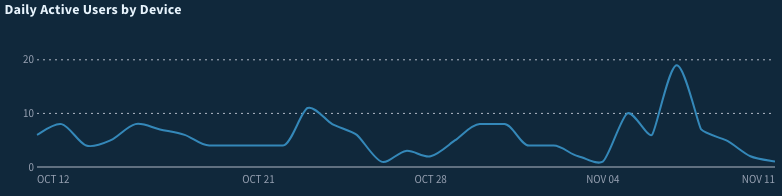
\includegraphics[width=\textwidth]{pfc/figuras/pilot-use.png}
    \caption{Uso diário da versão piloto do aplicativo}
    \label{fig:pilot-use}
\end{figure}

\subsection{Desenvolvimento do Produto}
O resultado da implementação da aplicação, no período contemplado neste PFC de aproximadamente 4 meses, contribuíram para grandes avanços no desenvolvimento do produto. A versão atual do aplicativo para o sistema iOS totaliza 33 telas principais de interação com o usuário (Figura \ref{fig:all-screens}). Estas interfaces permitem que os seguintes fluxos de atividade sejam realizados pelos usuários finais do produto:

\begin{itemize}
    \item Cadastro de academias
    \item Cadastro de treinadores
    \item Construção de agenda semanal de blocos para locação nas academias
    \item Acompanhamento diário de sessões de treino agendadas nas academias
    \item Visualização de dados semanais das academias em dashboard
    \item Visualização e edição de perfil das academias
    \item Busca por academias disponíveis em mapa dinâmico
    \item Adição de academias à seleção de favoritos
    \item Visualização de agenda diária dos treinadores
    \item Cancelamento e avaliação de sessões de treino
    \item Visualização e edição de perfil de treinador
    \item Visualização de dados semanais dos treinadores em dashboard
    \item Visualização de disponibilidade diária de blocos de academias através de calendário
    \item Agendamento de sessão de treino
\end{itemize}

\begin{figure}[H]
	\centering
    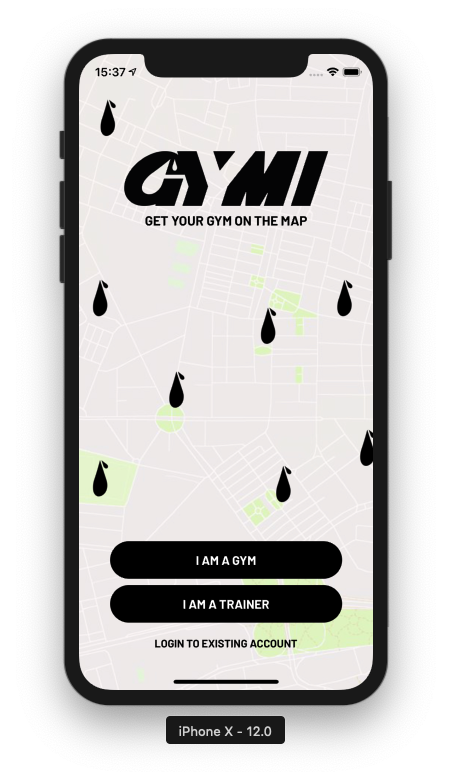
\includegraphics[width=0.14\textwidth]{pfc/figuras/landing.png}
    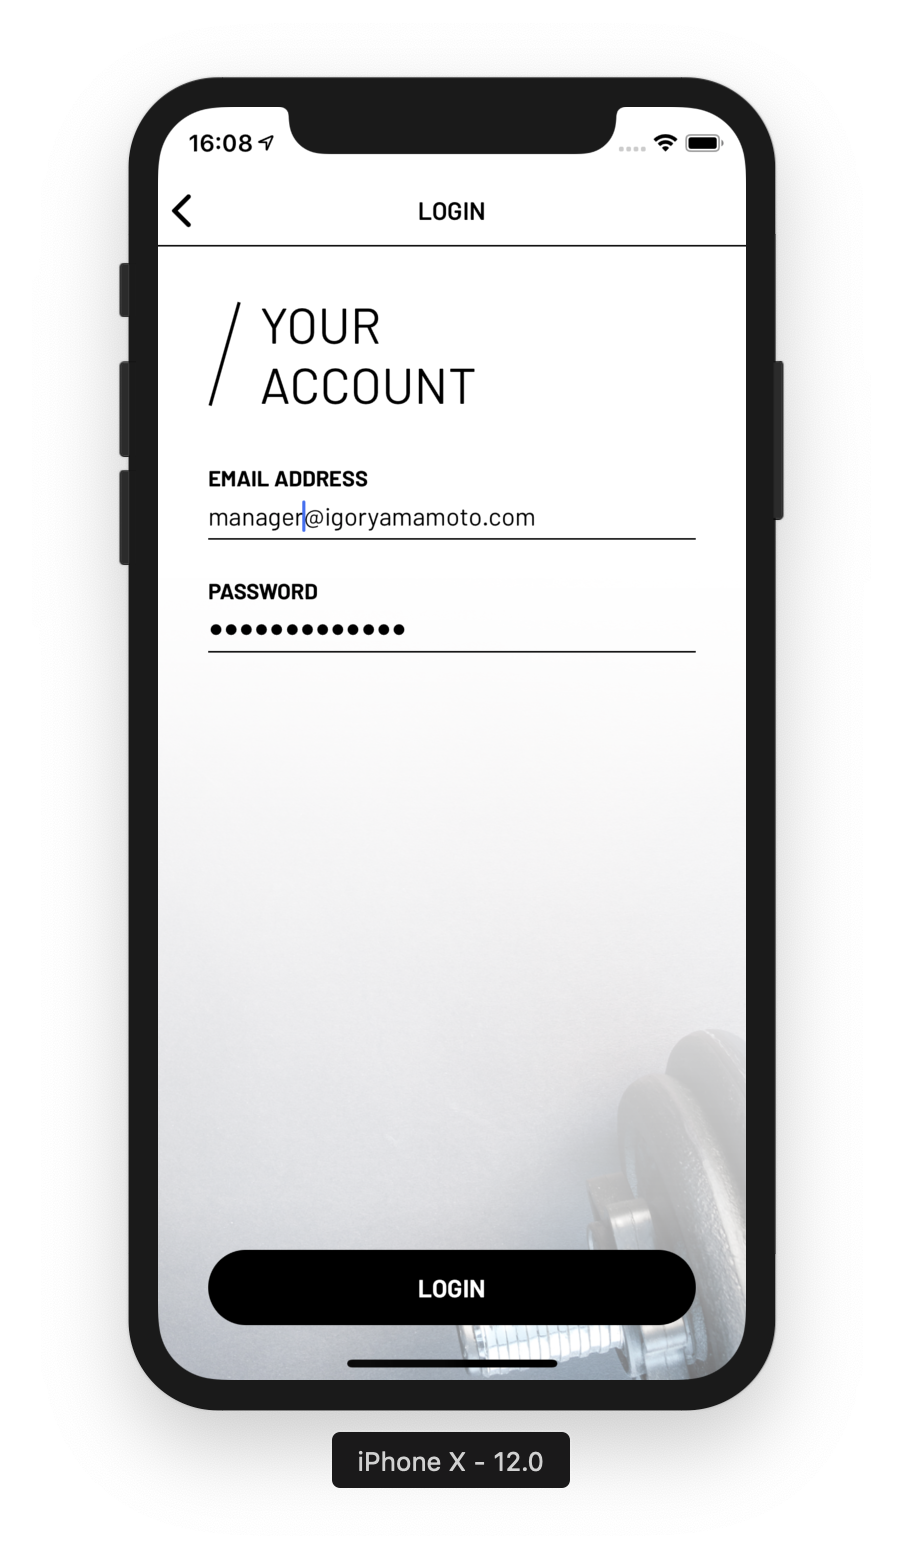
\includegraphics[width=0.14\textwidth]{pfc/figuras/login.png}
    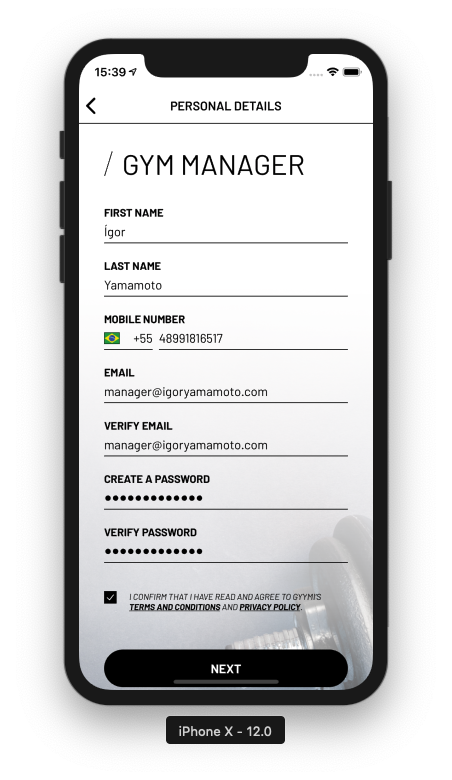
\includegraphics[width=0.14\textwidth]{pfc/figuras/register-manager.png}
    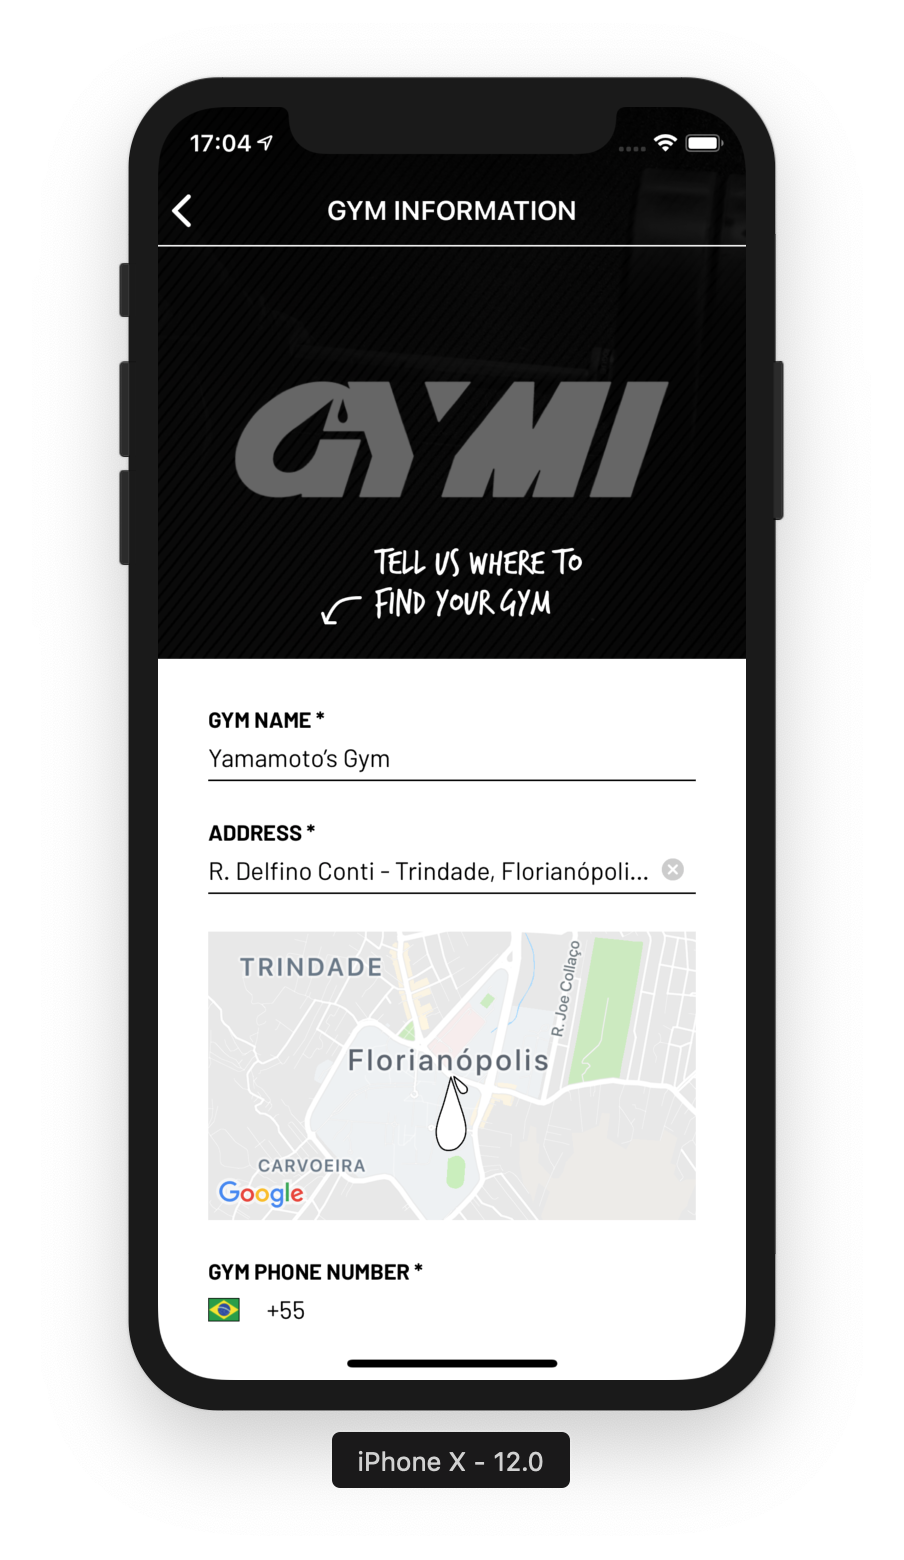
\includegraphics[width=0.14\textwidth]{pfc/figuras/register-gym-info.png}
    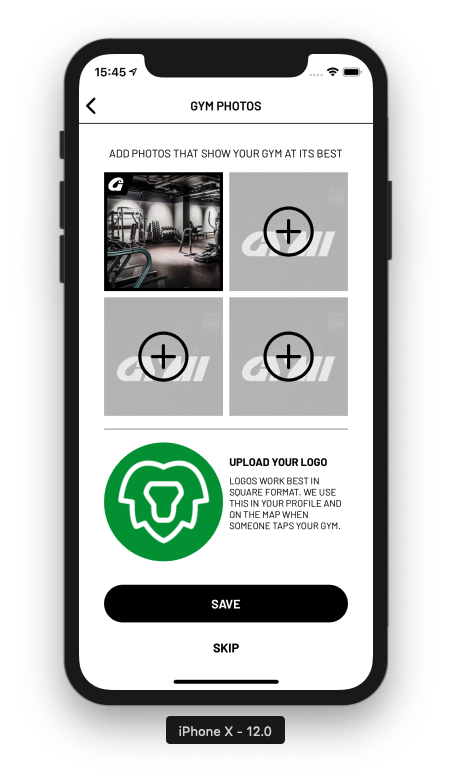
\includegraphics[width=0.14\textwidth]{pfc/figuras/register-gym-photos.png}
    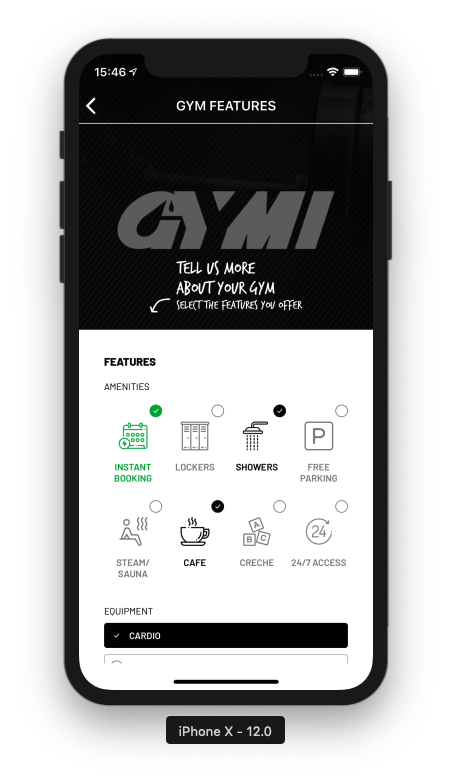
\includegraphics[width=0.14\textwidth]{pfc/figuras/register-gym-amenities.png}
    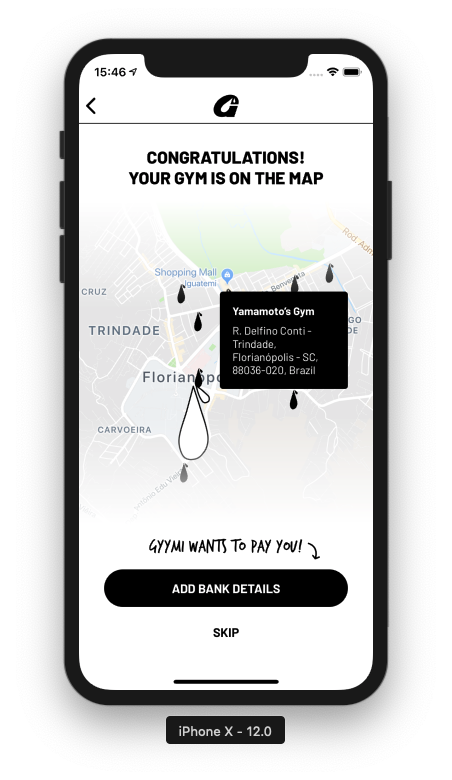
\includegraphics[width=0.14\textwidth]{pfc/figuras/gym-welcome.png}
    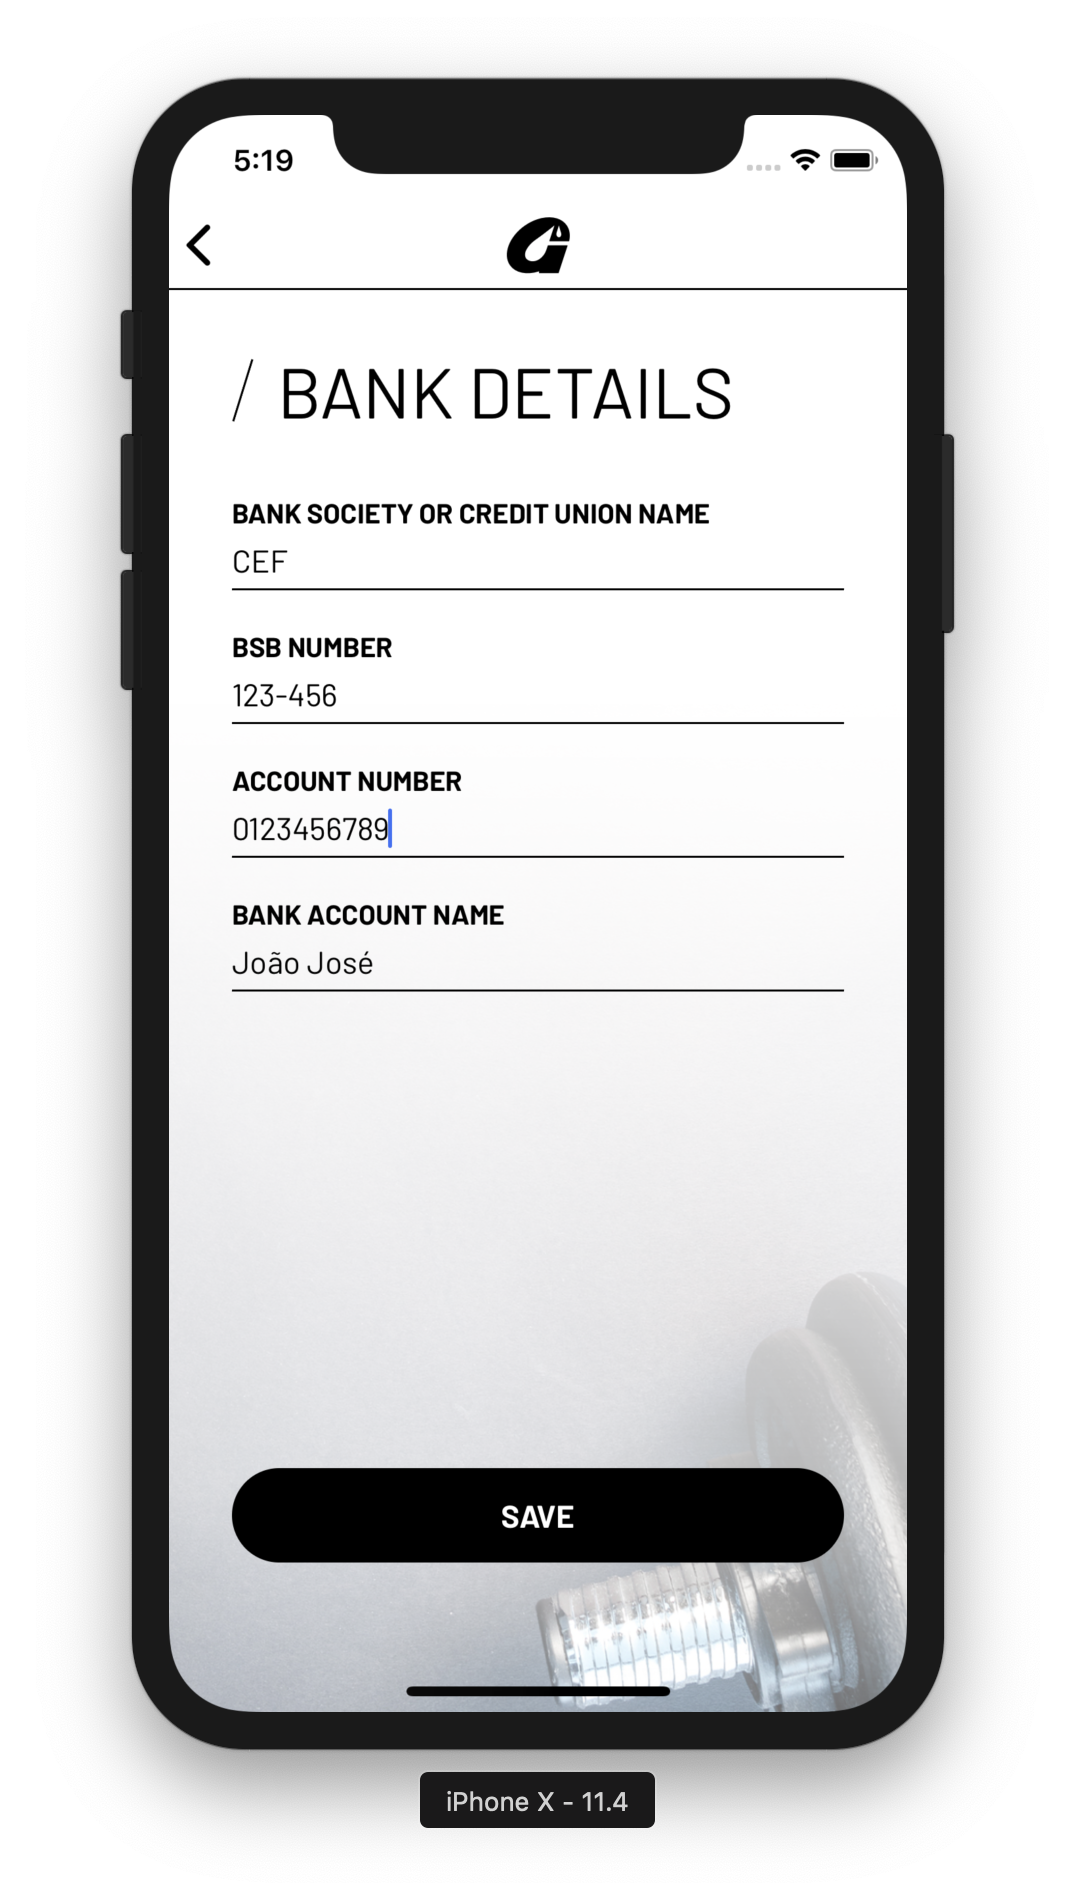
\includegraphics[width=0.14\textwidth]{pfc/figuras/bank-details.png}
    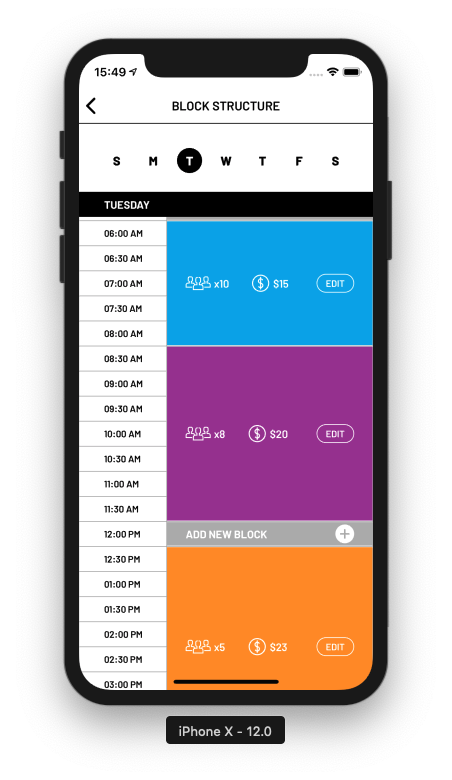
\includegraphics[width=0.14\textwidth]{pfc/figuras/gym-block-structure.png}
    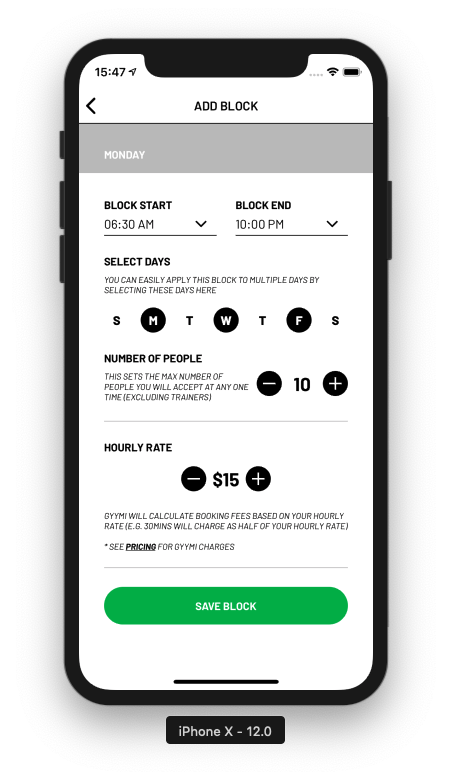
\includegraphics[width=0.14\textwidth]{pfc/figuras/gym-add-block.png}
    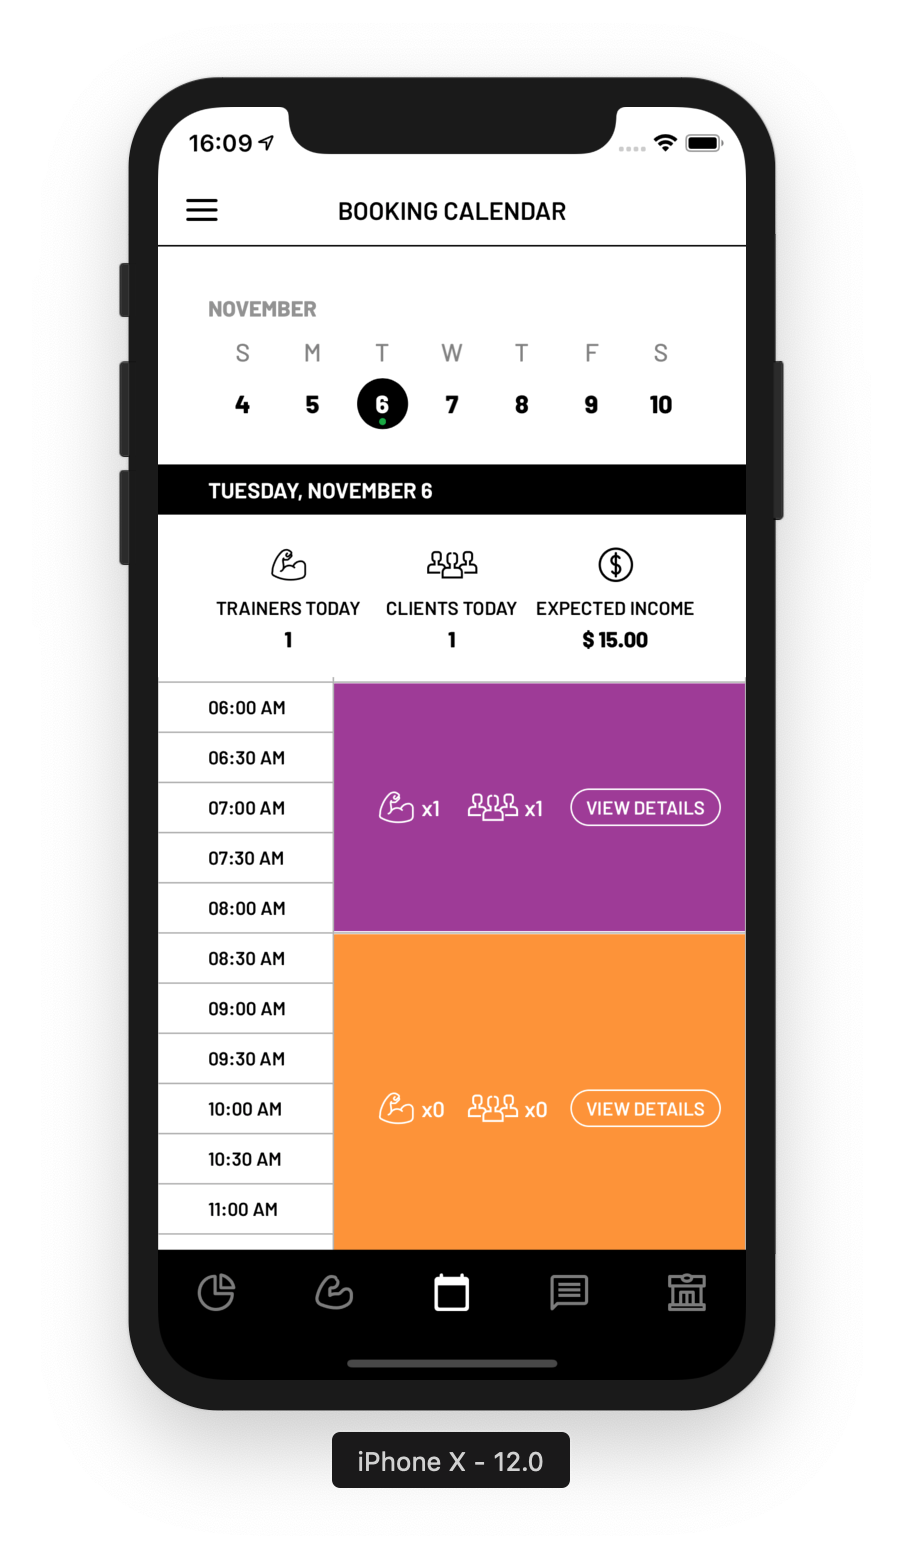
\includegraphics[width=0.14\textwidth]{pfc/figuras/gym-booking-calendar.png}
    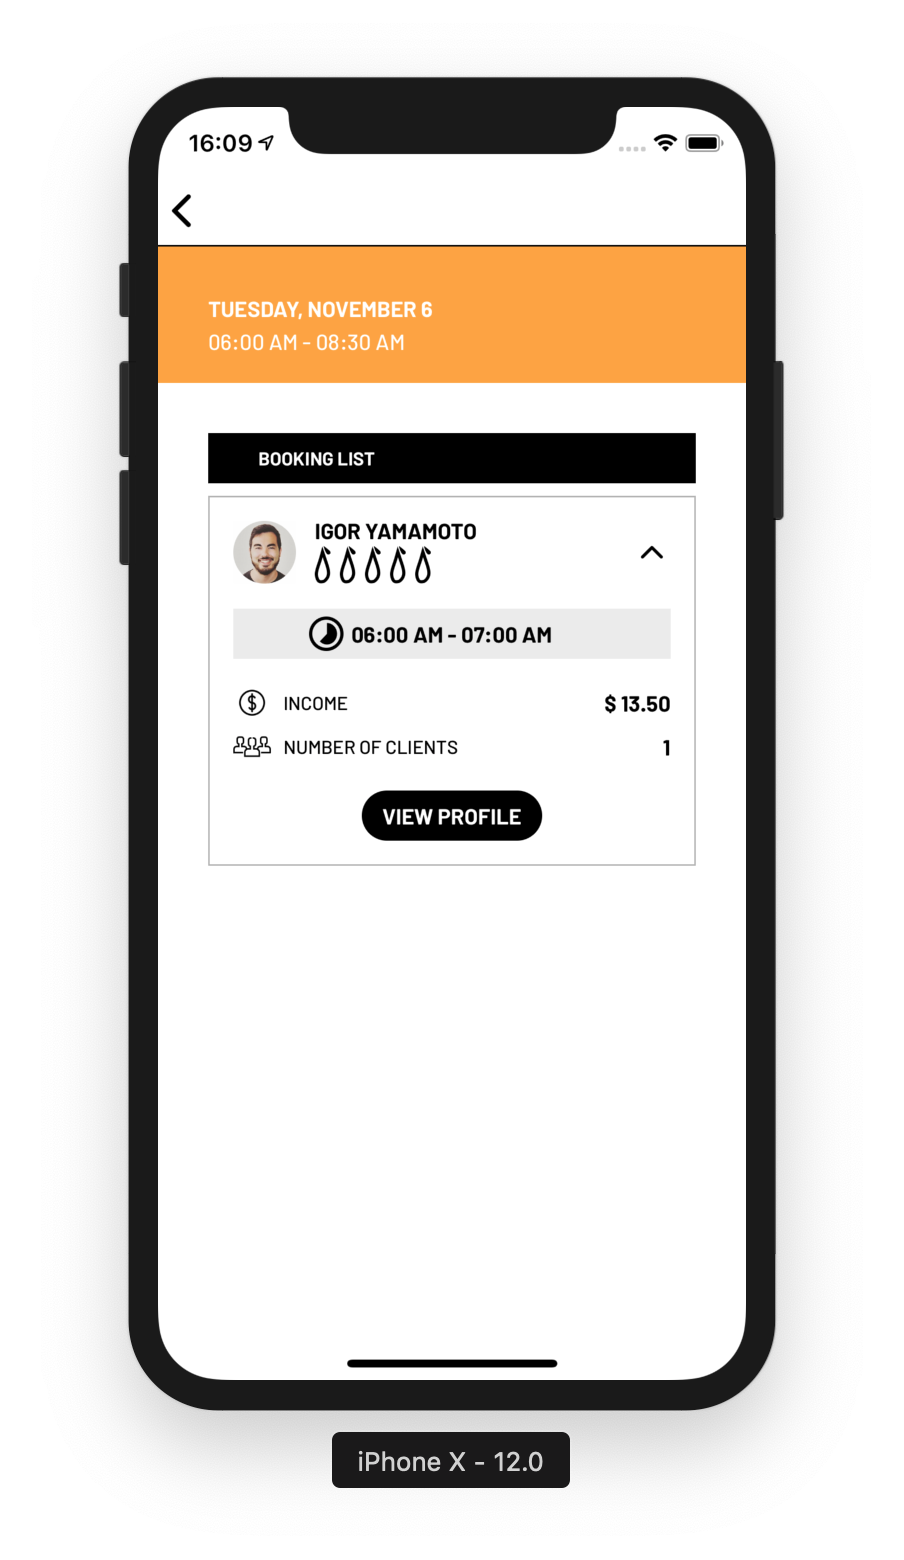
\includegraphics[width=0.14\textwidth]{pfc/figuras/gym-booking-detail.png}
    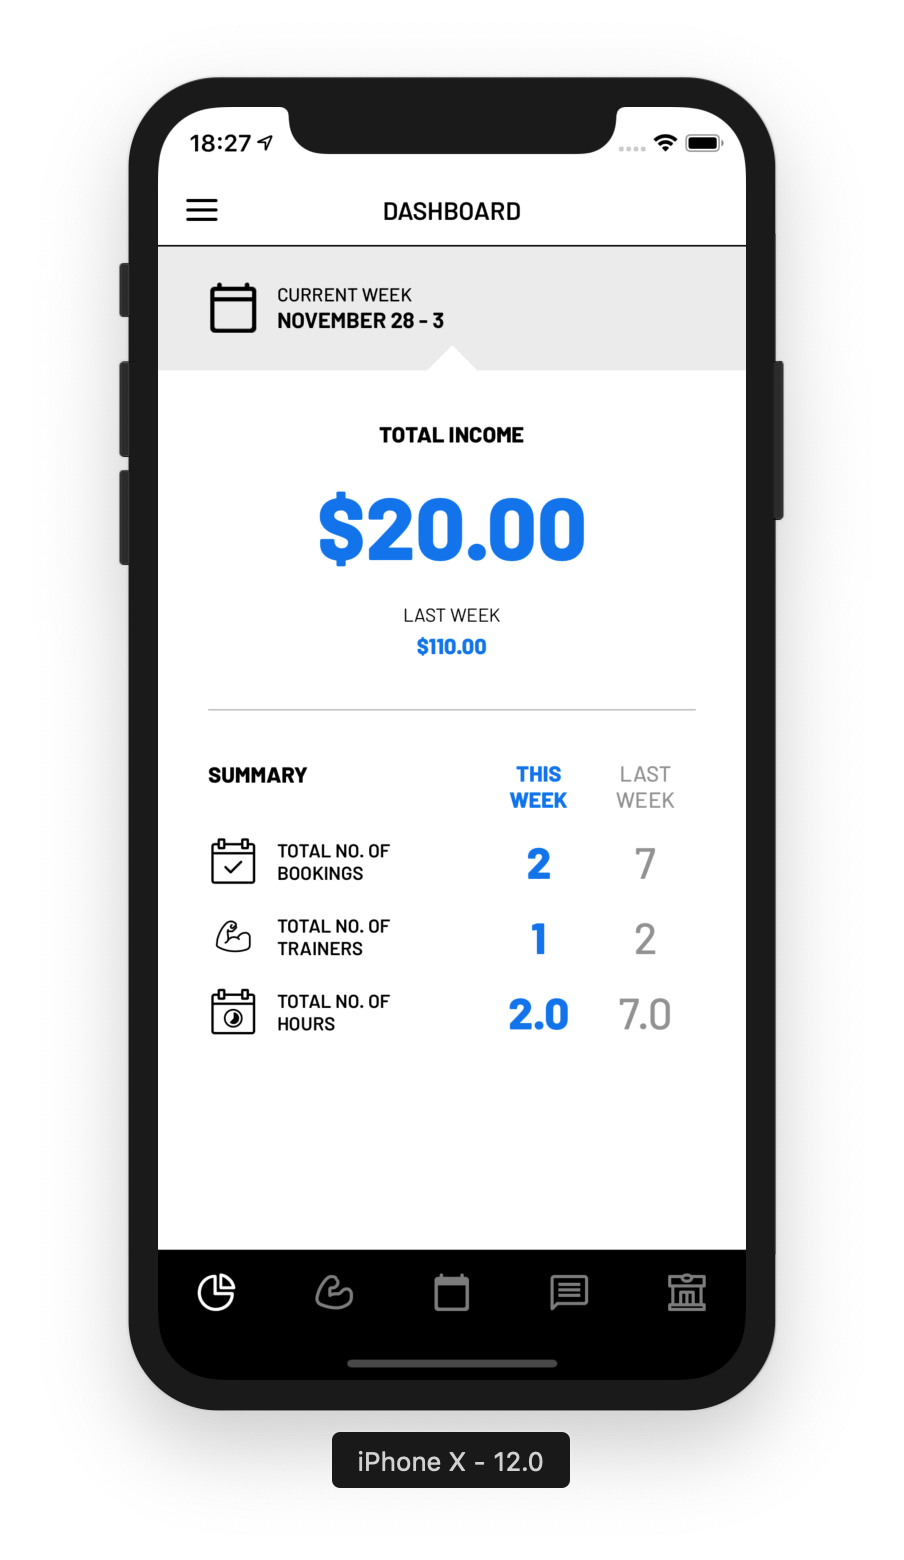
\includegraphics[width=0.14\textwidth]{pfc/figuras/gym-dashboard.png}
    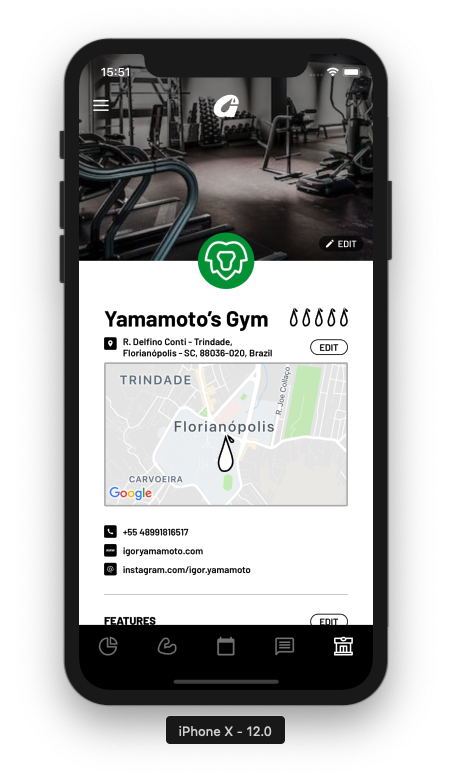
\includegraphics[width=0.14\textwidth]{pfc/figuras/gym-profile.png}
    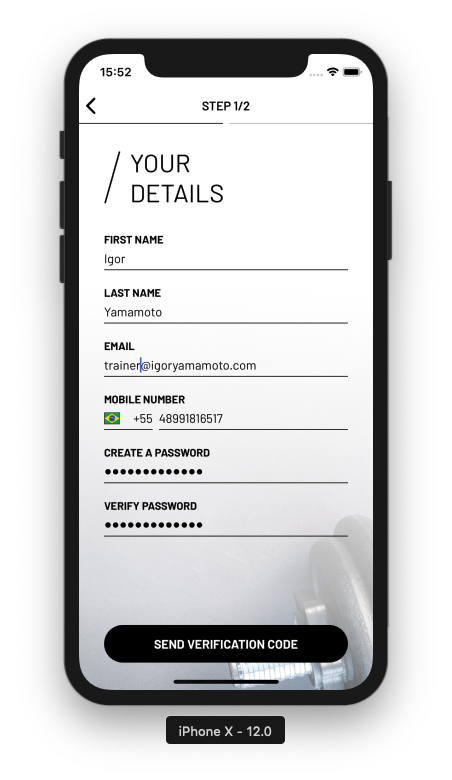
\includegraphics[width=0.14\textwidth]{pfc/figuras/register-trainer.png}
    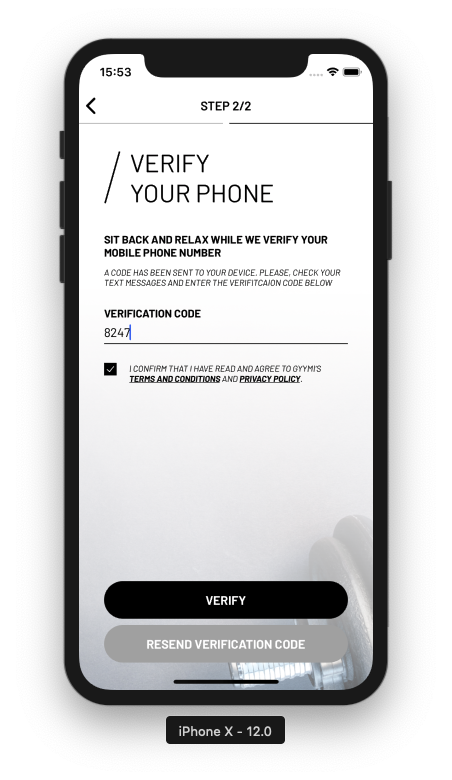
\includegraphics[width=0.14\textwidth]{pfc/figuras/register-trainer-verification.png}
    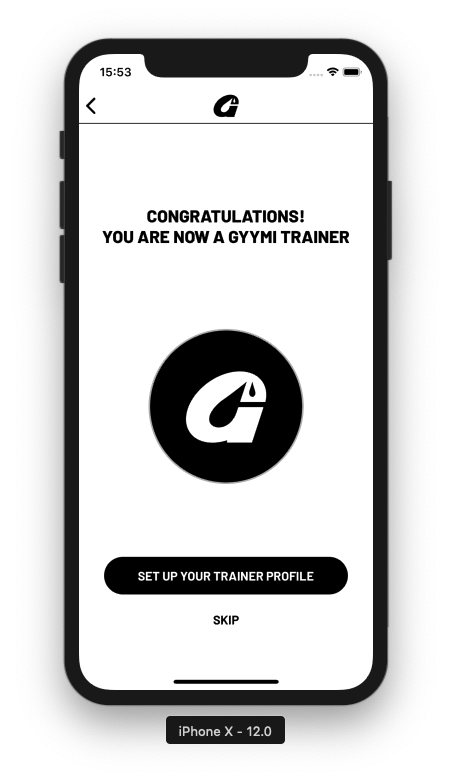
\includegraphics[width=0.14\textwidth]{pfc/figuras/tr-congratulations.png}
    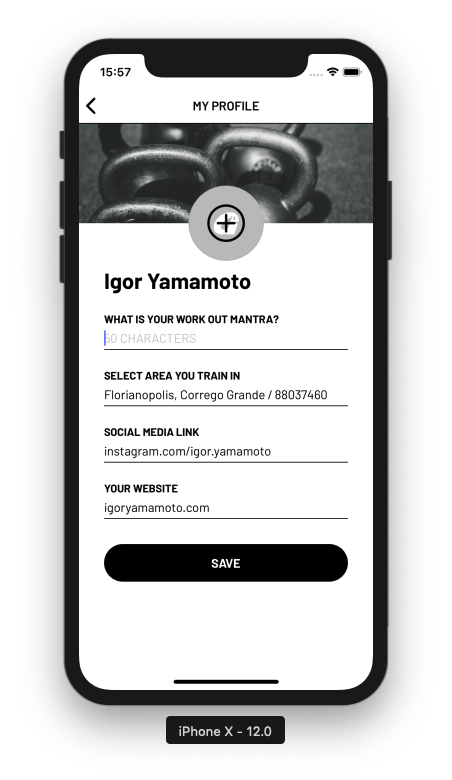
\includegraphics[width=0.14\textwidth]{pfc/figuras/tr-register-profile-1.png}
    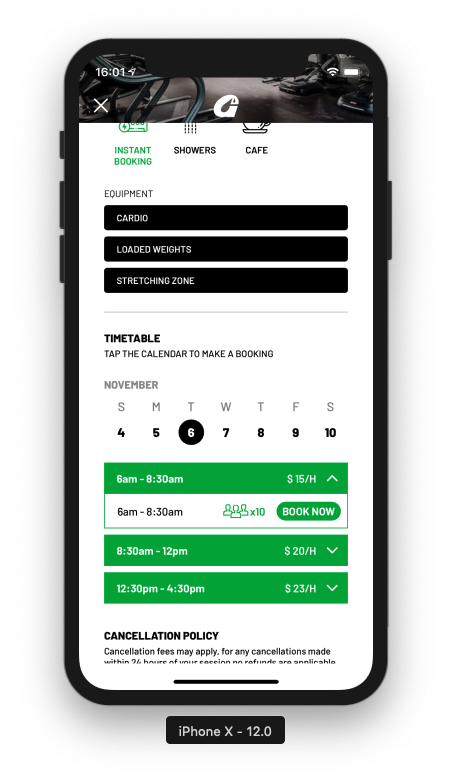
\includegraphics[width=0.14\textwidth]{pfc/figuras/tr-gym-profile-2.png}
    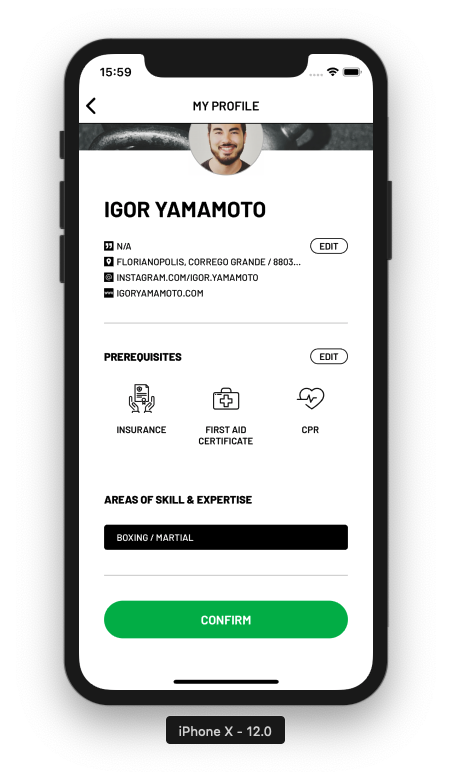
\includegraphics[width=0.14\textwidth]{pfc/figuras/tr-register-profile-3.png}
    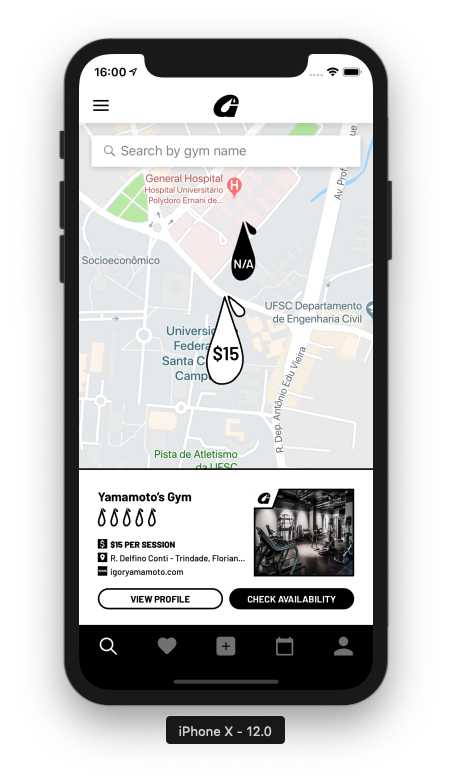
\includegraphics[width=0.14\textwidth]{pfc/figuras/tr-home-map.png}
    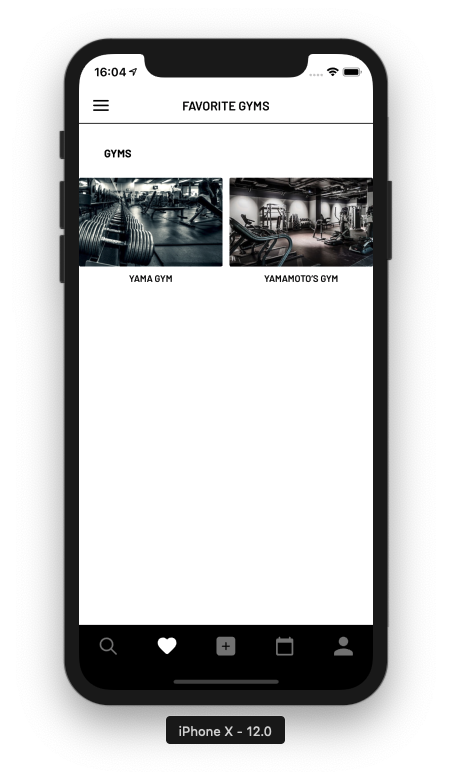
\includegraphics[width=0.14\textwidth]{pfc/figuras/tr-favorite.png}
    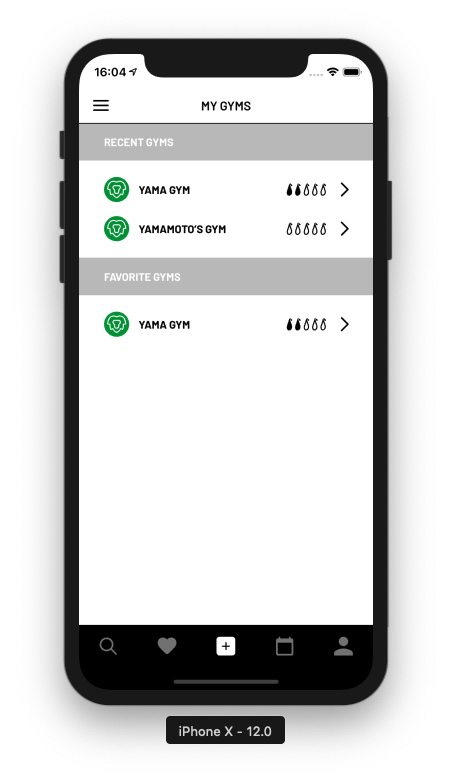
\includegraphics[width=0.14\textwidth]{pfc/figuras/tr-my-gyms.png}
    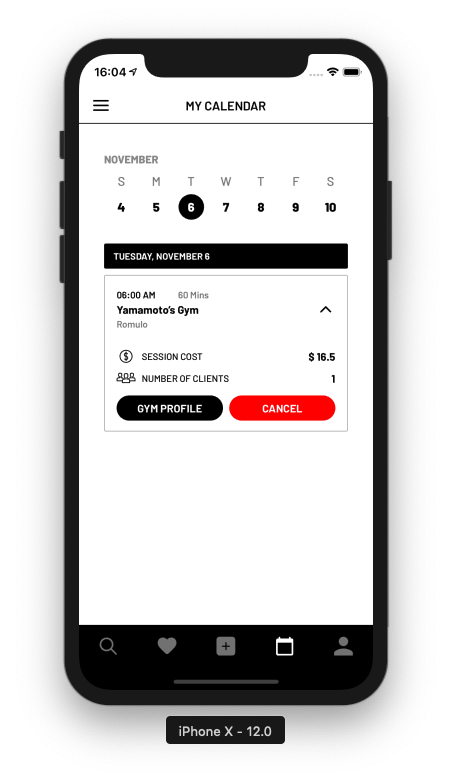
\includegraphics[width=0.14\textwidth]{pfc/figuras/tr-calendar.png}
    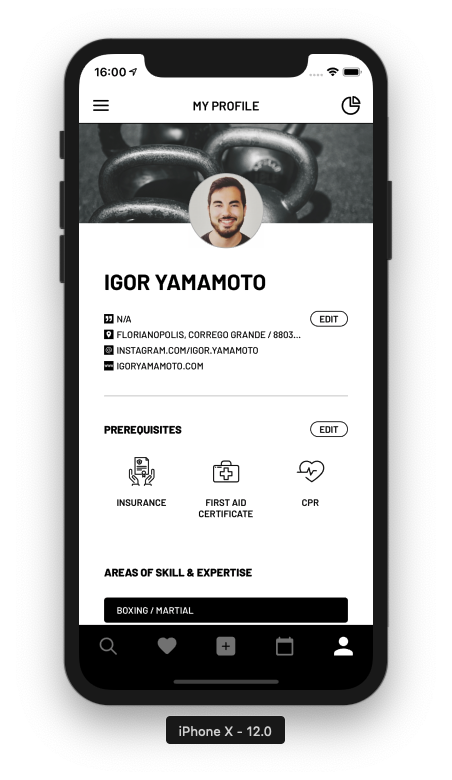
\includegraphics[width=0.14\textwidth]{pfc/figuras/tr-profile.png}
    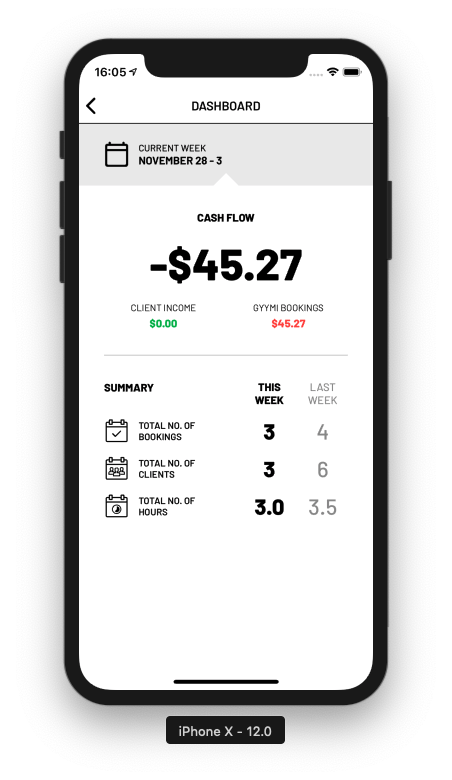
\includegraphics[width=0.14\textwidth]{pfc/figuras/tr-dashboard.png}
    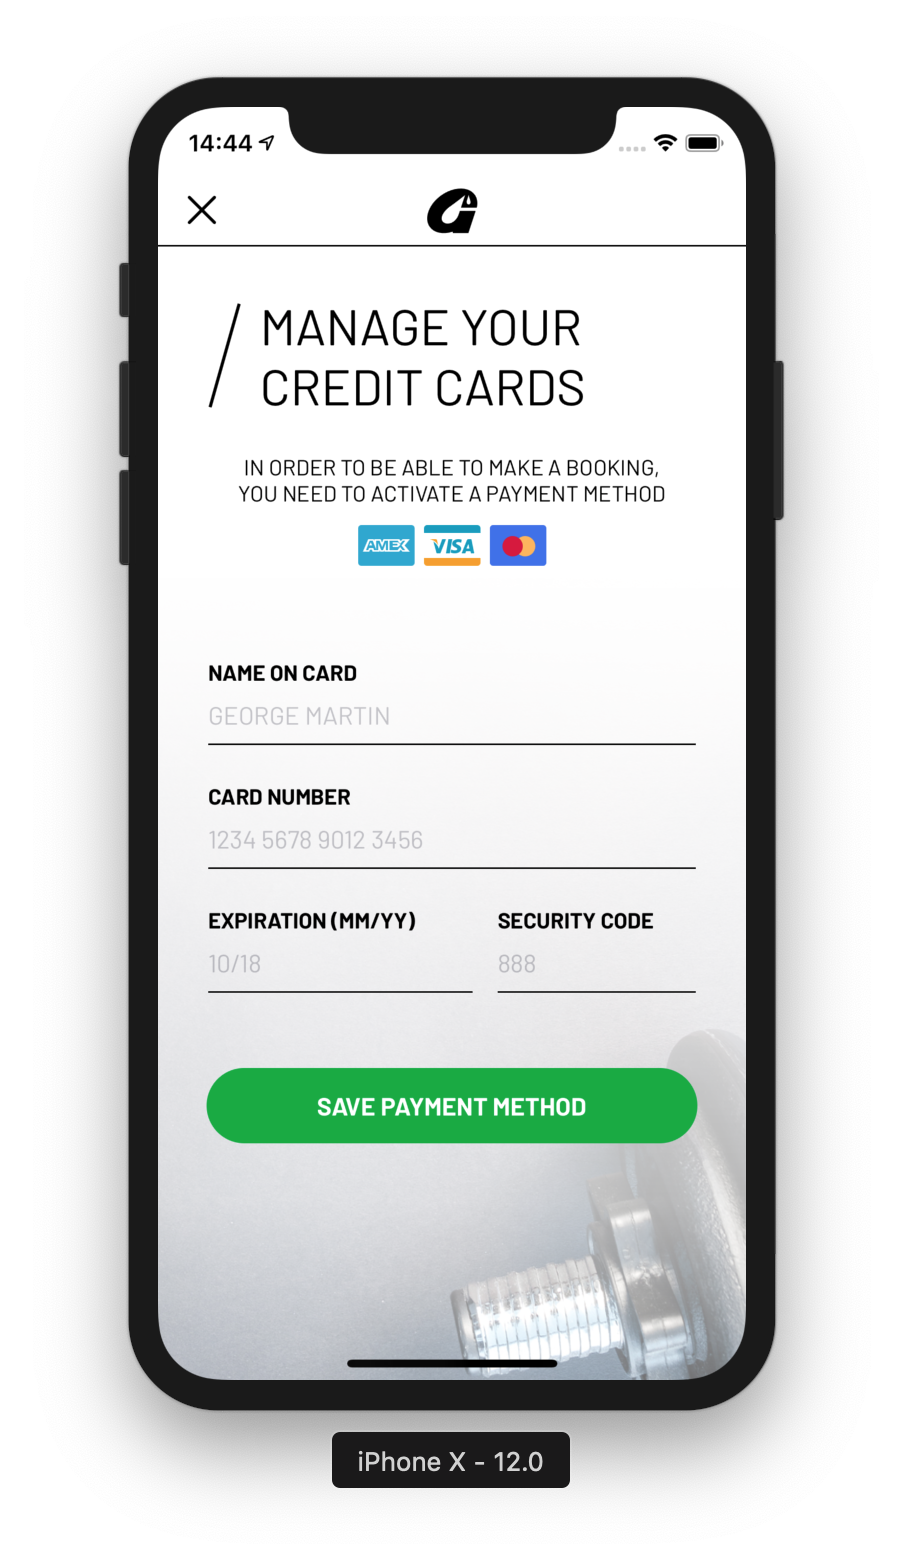
\includegraphics[width=0.14\textwidth]{pfc/figuras/add-card.png}
    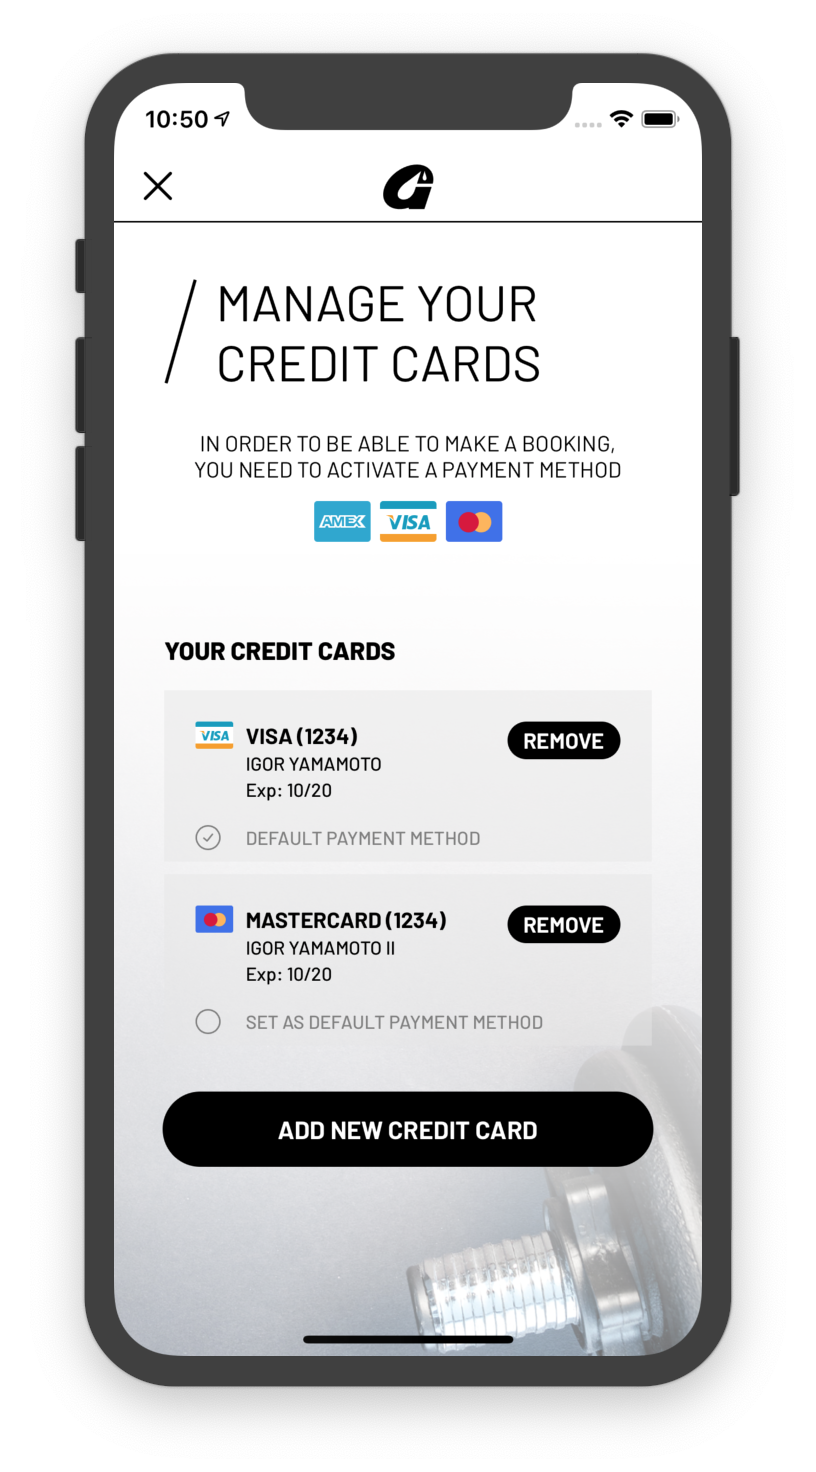
\includegraphics[width=0.14\textwidth]{pfc/figuras/manage-cards.png}
    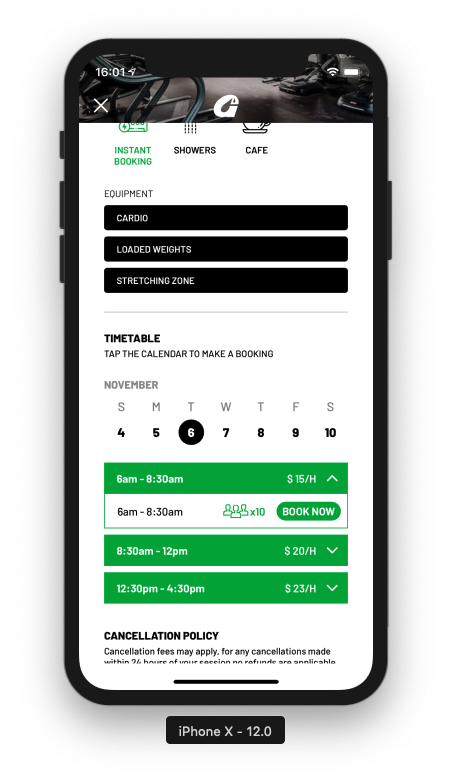
\includegraphics[width=0.14\textwidth]{pfc/figuras/tr-gym-profile-2.png}
    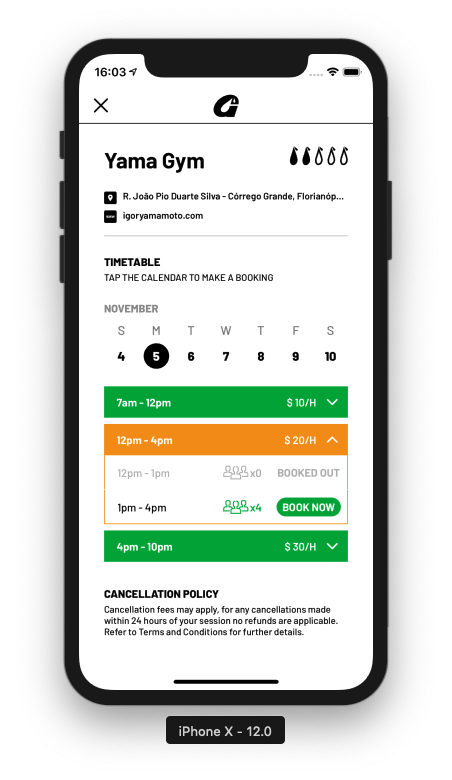
\includegraphics[width=0.14\textwidth]{pfc/figuras/tr-availability-2.png}
    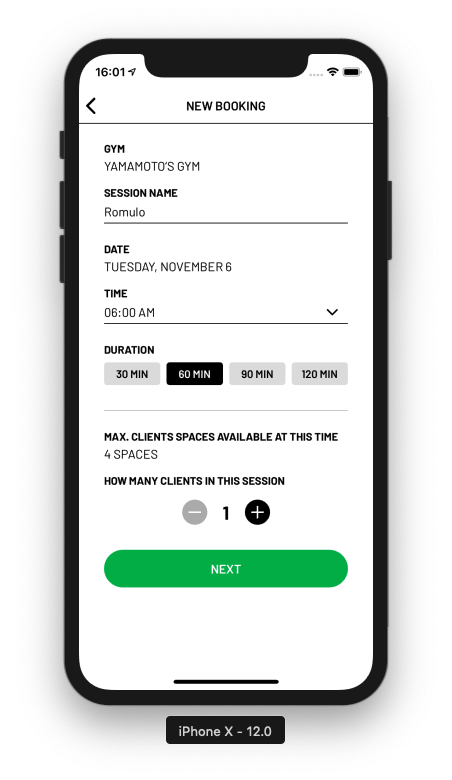
\includegraphics[width=0.14\textwidth]{pfc/figuras/tr-new-booking.png}
    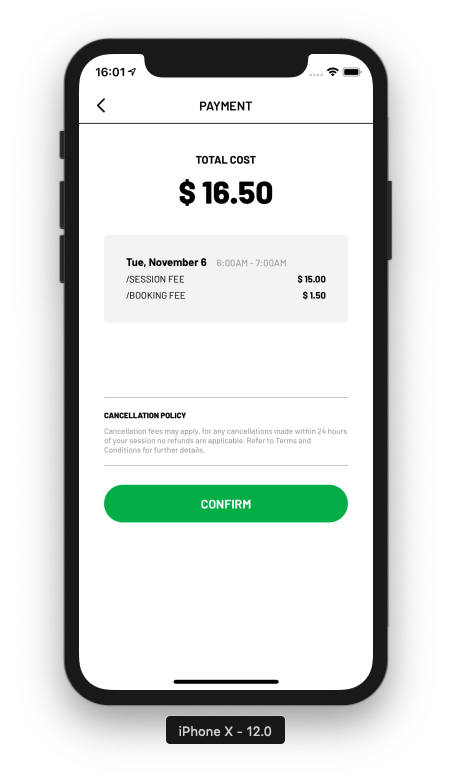
\includegraphics[width=0.14\textwidth]{pfc/figuras/tr-booking-payment.png}
    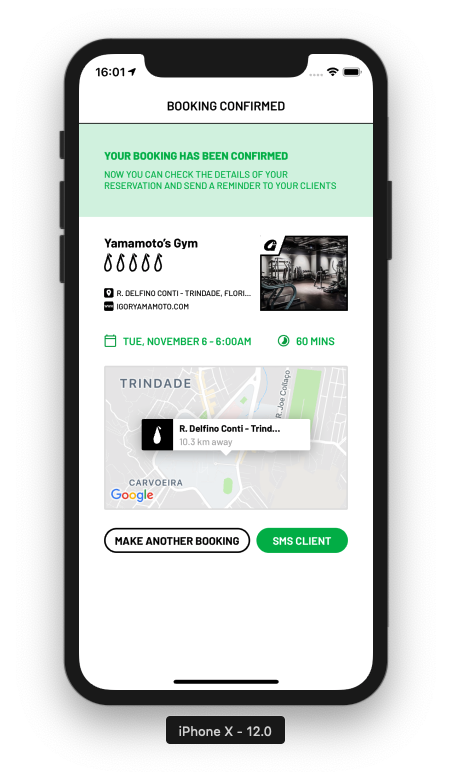
\includegraphics[width=0.14\textwidth]{pfc/figuras/tr-booking-confirmed.png}
    \caption{Todas as telas desenvolvidas para a versão piloto}
    \label{fig:all-screens}
\end{figure}

\section{Validação do Programa de Capacitação da Empresa}
O presente trabalho esteve inserido na empresa Jungle Devs como parte do programa de capacitação do autor. O programa de capacitação \textit{Academy} não havia sido concluído por nenhuma pessoa anteriormente. Portanto, um dos resultados obtidos por este PFC para a empresa é a validação do programa.

A proposta de conclusão de um projeto de aplicação prática real, em conjunto com um time de engenharia de software, foi efetuada com sucesso. O projeto do aplicativo Gyymi para o sistema iOS se mostrou eficaz para a capacitação do autor em projetos de aplicações \textit{mobile}. Isso se deve ao fato do aplicativo contemplar a maioria das funcionalidades recorrentes em aplicativos em produção no mercado, como cadastro e autenticação de usuários, navegação customizada por múltiplas telas e integração com sistemas de software terceiros.

Além de validar a etapa final do programa \textit{Academy}, na qual o projeto do aplicativo esteve inserido, o trabalho revelou bons resultados no que diz respeito às etapas anteriores. Esta afirmação é justificada a partir da análise da contribuição prática do autor para o projeto. A partir dos dados disponíveis no repositório do código fonte da aplicação (ver Figura \ref{fig:github-stats}), é possível concluir que o autor teve contribuições significativas desde o começo do projeto. Os dados indicam a contribuição do autor em $70\%$ das linhas de código modificadas durante o projeto, totalizando $55408$ alterações. Além disso, o autor teve contribuição em $74\%$ dos incrementos de versão do código (\textit{commits}), totalizando $699$ mensagens de incremento salvas. Assim, é possível concluir que as etapas iniciais do programa de capacitação foram efetivas para a aprendizagem de conceitos práticos de projeto.

\begin{figure}[H]
    \centering
    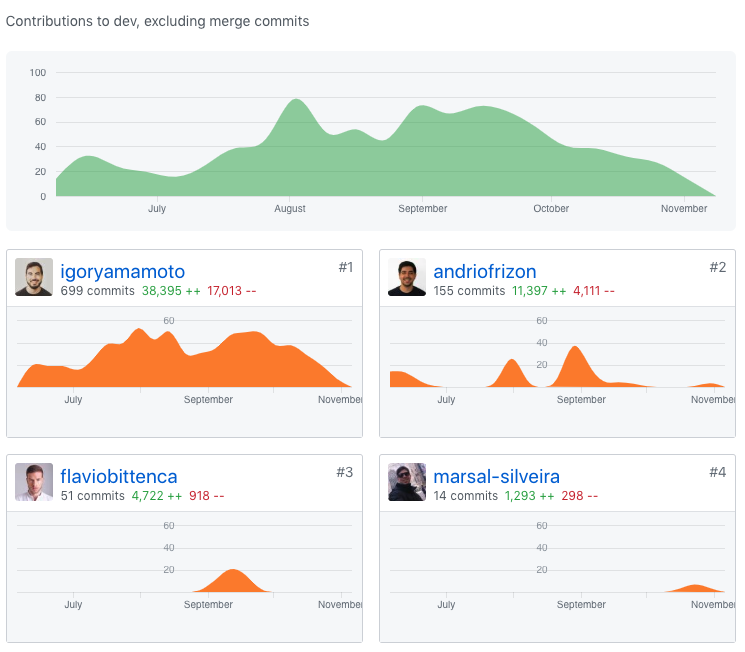
\includegraphics[width=\textwidth]{pfc/figuras/github-stats.png}
    \caption{Dados de contribuição no projeto do aplicativo iOS por membro do time}
    \label{fig:github-stats}
\end{figure}

\section{Testes Automatizados}
